\documentclass[convert={density=600,outext=.png,convertexe={magick}},tikz,crop=true,border=0pt]{standalone}

\usepackage{tikz}
\usepackage{xifthen}
\usetikzlibrary{calc}

\begin{document}

% Draw a little slope calculation box with +/-0.5 around:
%   #1=ptx, #2=pty, #3=slope
\def\drawQtStepSlope#1#2#3{ 	
	\ifthenelse{\lengthtest{#3pt<1pt}}{%
			\draw [color=red, ultra thick] ({#1-0.5, #2-0.5*#3}) -- ({#1+0.5, #2+0.5*#3});
			\node[draw,circle,inner sep=1pt,fill,color=red] at (#1,#2) {};
			\draw [style=help lines, xstep=0.125, ystep=0.125]      (#1-0.501,#2-0.501) grid +(1.01,1.01);
			\node [above] at (#1,#2+0.5) {\footnotesize $\!\!\!\!\! f'(#1)=#3$};
		}{
			\draw [color=red, ultra thick] ({#1-0.5/#3, #2-0.5}) -- ({#1+0.5/#3, #2+0.5});
			\node[draw,circle,inner sep=1pt,fill,color=red] at (#1,#2) {};
			\draw [style=help lines, xstep=0.125, ystep=0.125]      (#1-0.501,#2-0.501) grid +(1.01,1.01);
			\node [above] at (#1,#2+0.5) {\footnotesize $ \!\!\!\!\!  f'(#1)=#3$};
		}
	}

\pagestyle{empty}

% Keep x-scale the same, but halve y-scale (factor 2 change) so the plot looks the same
% after replacing (1/2)x^2 by x^2.
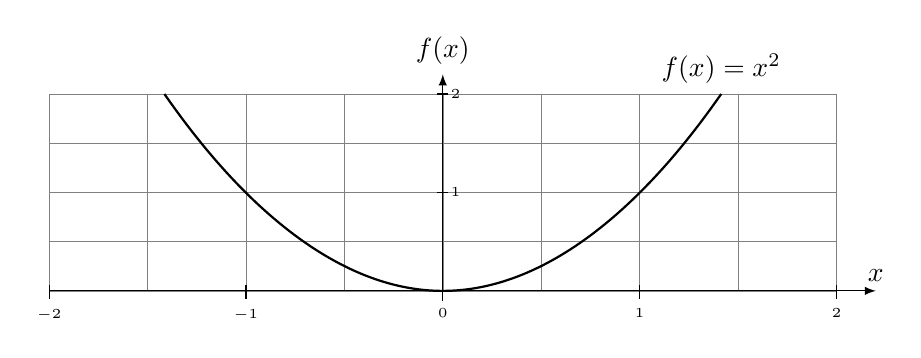
\begin{tikzpicture}[x=2.5cm,y=1.25cm]  % y is half of x: previously both effectively 2cm

	\coordinate (XAxisMin) at (-2,0);
	\coordinate (XAxisMax) at (2.2,0);
	\coordinate (YAxisMin) at (0,-0.1);
	\coordinate (YAxisMax) at (0,2.2); % keep same numeric limits; y-unit is scaled

	\coordinate (OneOne) at (1, 1);

	\draw [style=help lines,step=0.5] (-2,0) grid (2,2);	
	\draw[-> , >=latex]  (XAxisMin) --  (XAxisMax) node [above] {$x$};
	\draw[-> , >=latex] (YAxisMin) -- (YAxisMax) node [above] {$f(x)$};

	\foreach \x/\xtext in {-2/-2, -1/-1, 0/0, 1/1, 2/2}
		\draw[shift={(\x,0)}] (0pt,2pt) -- (0pt,-3pt) node[below] {\tiny $\xtext$};

	\foreach \y/\ytext in {1/1, 2/2}
		\draw[shift={(0,\y)}] (2pt,0pt) -- (-2pt,0pt) node[right, xshift=0.5mm] {\tiny $\ytext$};

	% f(x)=x^2, but with y-scale halved so it has the same visual shape as before.
	\draw [thick] (-1.41421356,2) parabola bend (0,0) (1.41421356,2)
		node[above] {$f(x)=x^2$};

	% Tangents: points moved to lie on y=x^2 in the new (scaled) coordinate system.
	% At x=1: y=1, slope=2
	\drawQtStepSlope{1}{1}{2};

	% At x=-0.5: y=0.25, slope=-1
	\drawQtStepSlope{-0.5}{0.25}{-1};

\end{tikzpicture}

\end{document}
